\section{\acl{RL} dalam Sistem Kontrol}

\ac{RL}, sebagai kerangka agen otonom, merupakan salah satu alternatif yang bagus sebagai sistem komplementer maupun utama dari sebuah sistem kontrol. Hal tersebut merupakan akibat dari kapabilitas \ac{RL} untuk menentukan sinyal kontrol. yang dekat ke nilai optimal dengan cara \textit{trial-and-error} \parencite{vichugov2005application}. Secara umum, sistem RL yang dikembangkan dapat menjadi tambahan \textit{feedback loop} dari sebuah sistem kontrol diskrit yang dapat diilustrasikan pada Gambar \ref{fig:RL-loop-kontrol}.


\begin{figure}[H]
	\centering
	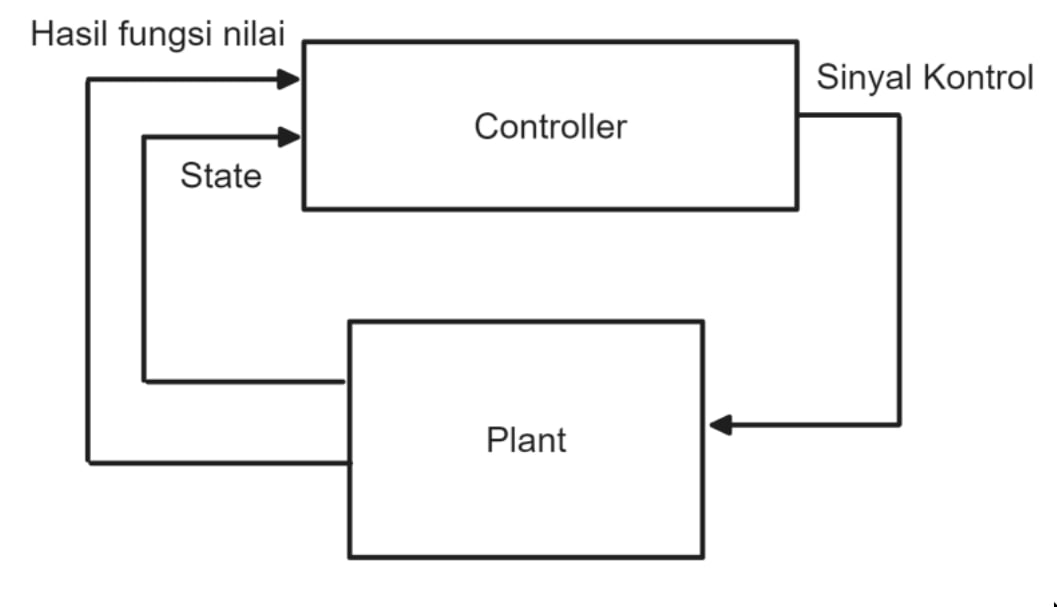
\includegraphics[width=0.8\textwidth]{chapter-2/RL-kontrol-loop.jpg}
	\caption{Diagram Feedback Loop \ac{RL} pada Sistem Kontrol \parencite{vichugov2005application}}
	\label{fig:RL-loop-kontrol}
\end{figure}

Pada Gambar \ref{fig:RL-loop-kontrol}, digambarkan sebuah kerangka \ac{RL} yang menggunakan keluaran sinyal kontrol sebagai aksi, keluaran \textit{plant} sebagai \textit{state}, dengan fungsi nilai yang diformulasikan bersesuaian dengan fisis yang ada pada \textit{plant}. Permasalahan \textit{cart pole balancing} \parencite{nagendra2017comparison} merupakan salah satu contoh sistem kontrol klasik yang marak digunakan untuk \textit{benchmarking} performa agen \ac{RL}. Berikut, pada Gambar \ref{fig:cartpole-illustration}, merupakan ilustrasi dari permasalahan \textit{cart pole balancing}.

\begin{figure}[h]
	\centering
	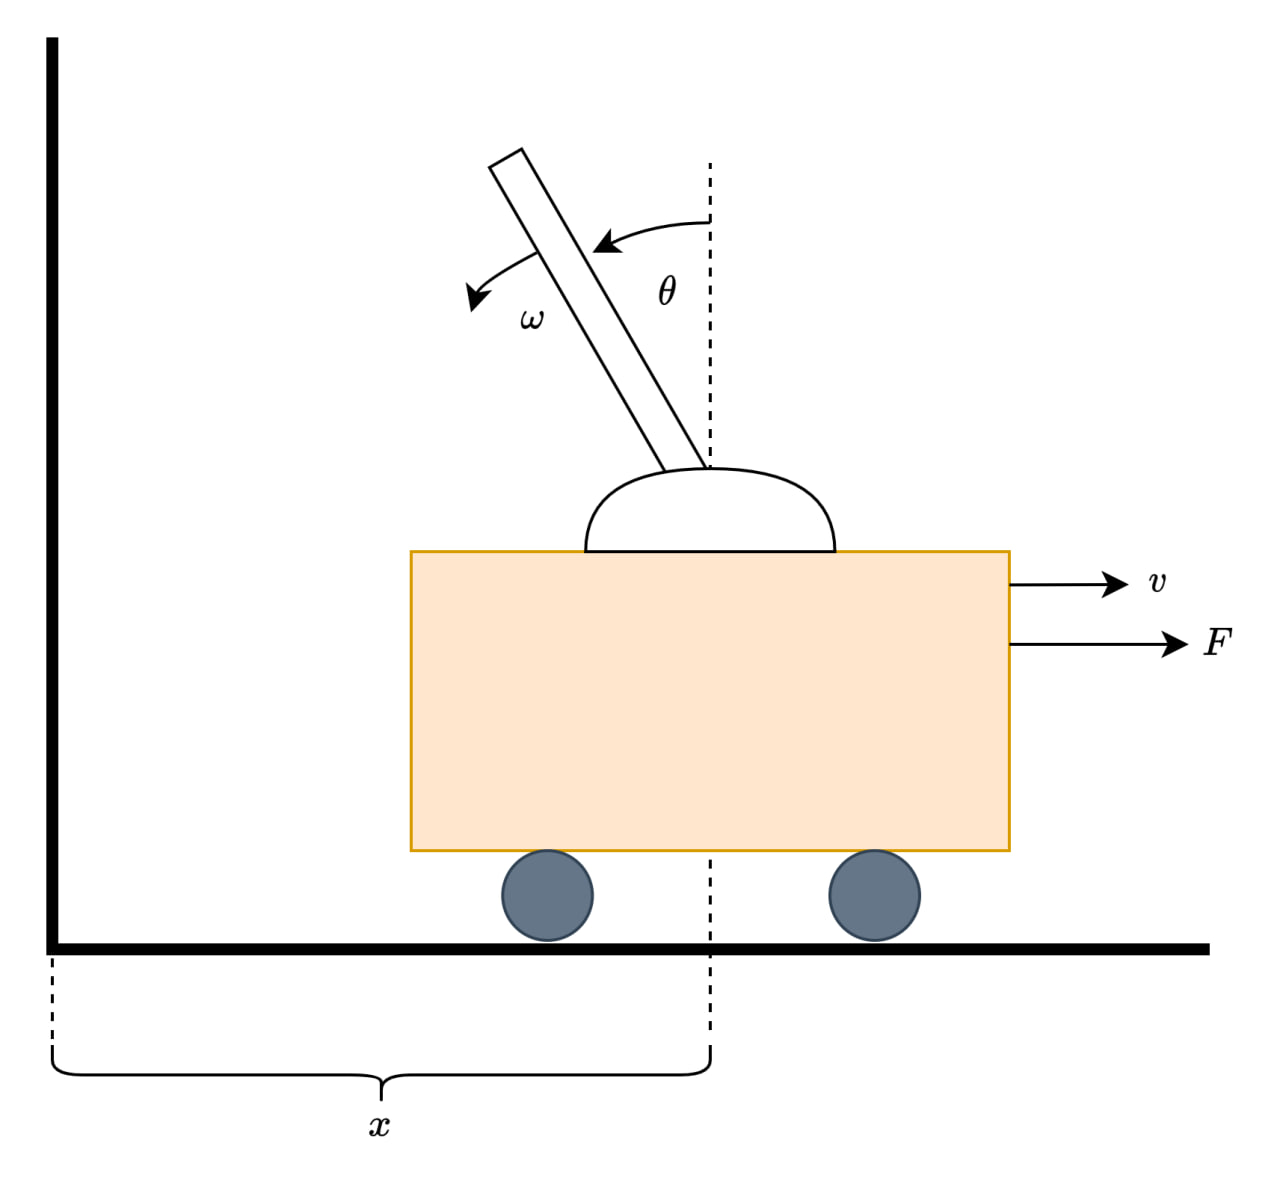
\includegraphics[width=0.6\textwidth]{chapter-2/cartpole-illustration.jpg}
	\caption{Ilustrasi Permasalahan \textit{Cart Pole Balancing}}
	\label{fig:cartpole-illustration}
\end{figure}

Pada sistem fisis sederhana Gambar \ref{fig:cartpole-illustration}, didefinisikan masing-masing variabel dari kerangka \ac{RL} sebagai berikut.

\begin{enumerate}
	\item \textit{State}: \(\theta\), \(\omega\), \(v\), dan \(x\)
	\item Aksi: \(F\)
\end{enumerate}

Kasus permasalahan \textit{Cart Pole Balancing}, sebagaimana kasus kontrol klasik lainnya, memerlukan sistem komputasi yang memiliki \textit{time delay} (\(t_d\)) yang kecil bila diimplementasikan pada sistem nyata. Bila \(t_d\) terlalu besar, maka sistem dapat menjadi tidak stabil sehingga tidak berhasil dikontrol oleh perhitungan dari agen \ac{RL}.

Seiring dengan semakin maraknya perkembangan \ac{RL}, sudah banyak kasus yang mengadopsi kerangka ini untuk digunakan pada sistem kontrol yang lebih kompleks [1, 2, 3]. Sehingga, \ac{RL} dapat tetap digunakan tanpa mengakibatkan ketidakstabilan pada sistem kontrol, maka diperlukan mekanisme universal yang dapat digunakan untuk mempercepat iterasi perhitungan RL pada \textit{processor} komputer.
